

\section{Interactive Analysis}
\label{sec:app_err_analysis}

While our use of \sysname has so far relied on automatic selection of counterfactuals, we show in this section how an analyst can benefit from \emph{multiple} counterfactuals per $x$, make use of controlled generation for more advanced analysis, and extract general patterns from individual observations.
Our use case is counterfactual error analysis~\cite{wu2019errudite} of RoBERTa finetuned on \nli (used in \S\ref{subsec:contrast_set}), although the techniques are generally applicable.

There is a known correlation between the label \emph{Contradiction} and hypotheses with negation in \nli datasets~\cite{gururangan2018annotation}, which may cause models to fail on non-contradiction negations.
We explore this in Figure~\ref{fig:err_analysis}A by generating counterfactual hypotheses for a random \emph{Neutral} instance, conditioning only on the original $x$ and the \texttt{negation} \tagstr.
While the first two counterfactuals display this failure mode, there is a surprising inconsistency in model behavior between ``not'' and ``n't''.
We note that manual analysis may not explore these three negation forms, and thus not surface this puzzling behavior.

\begin{figure}[t]
\centering
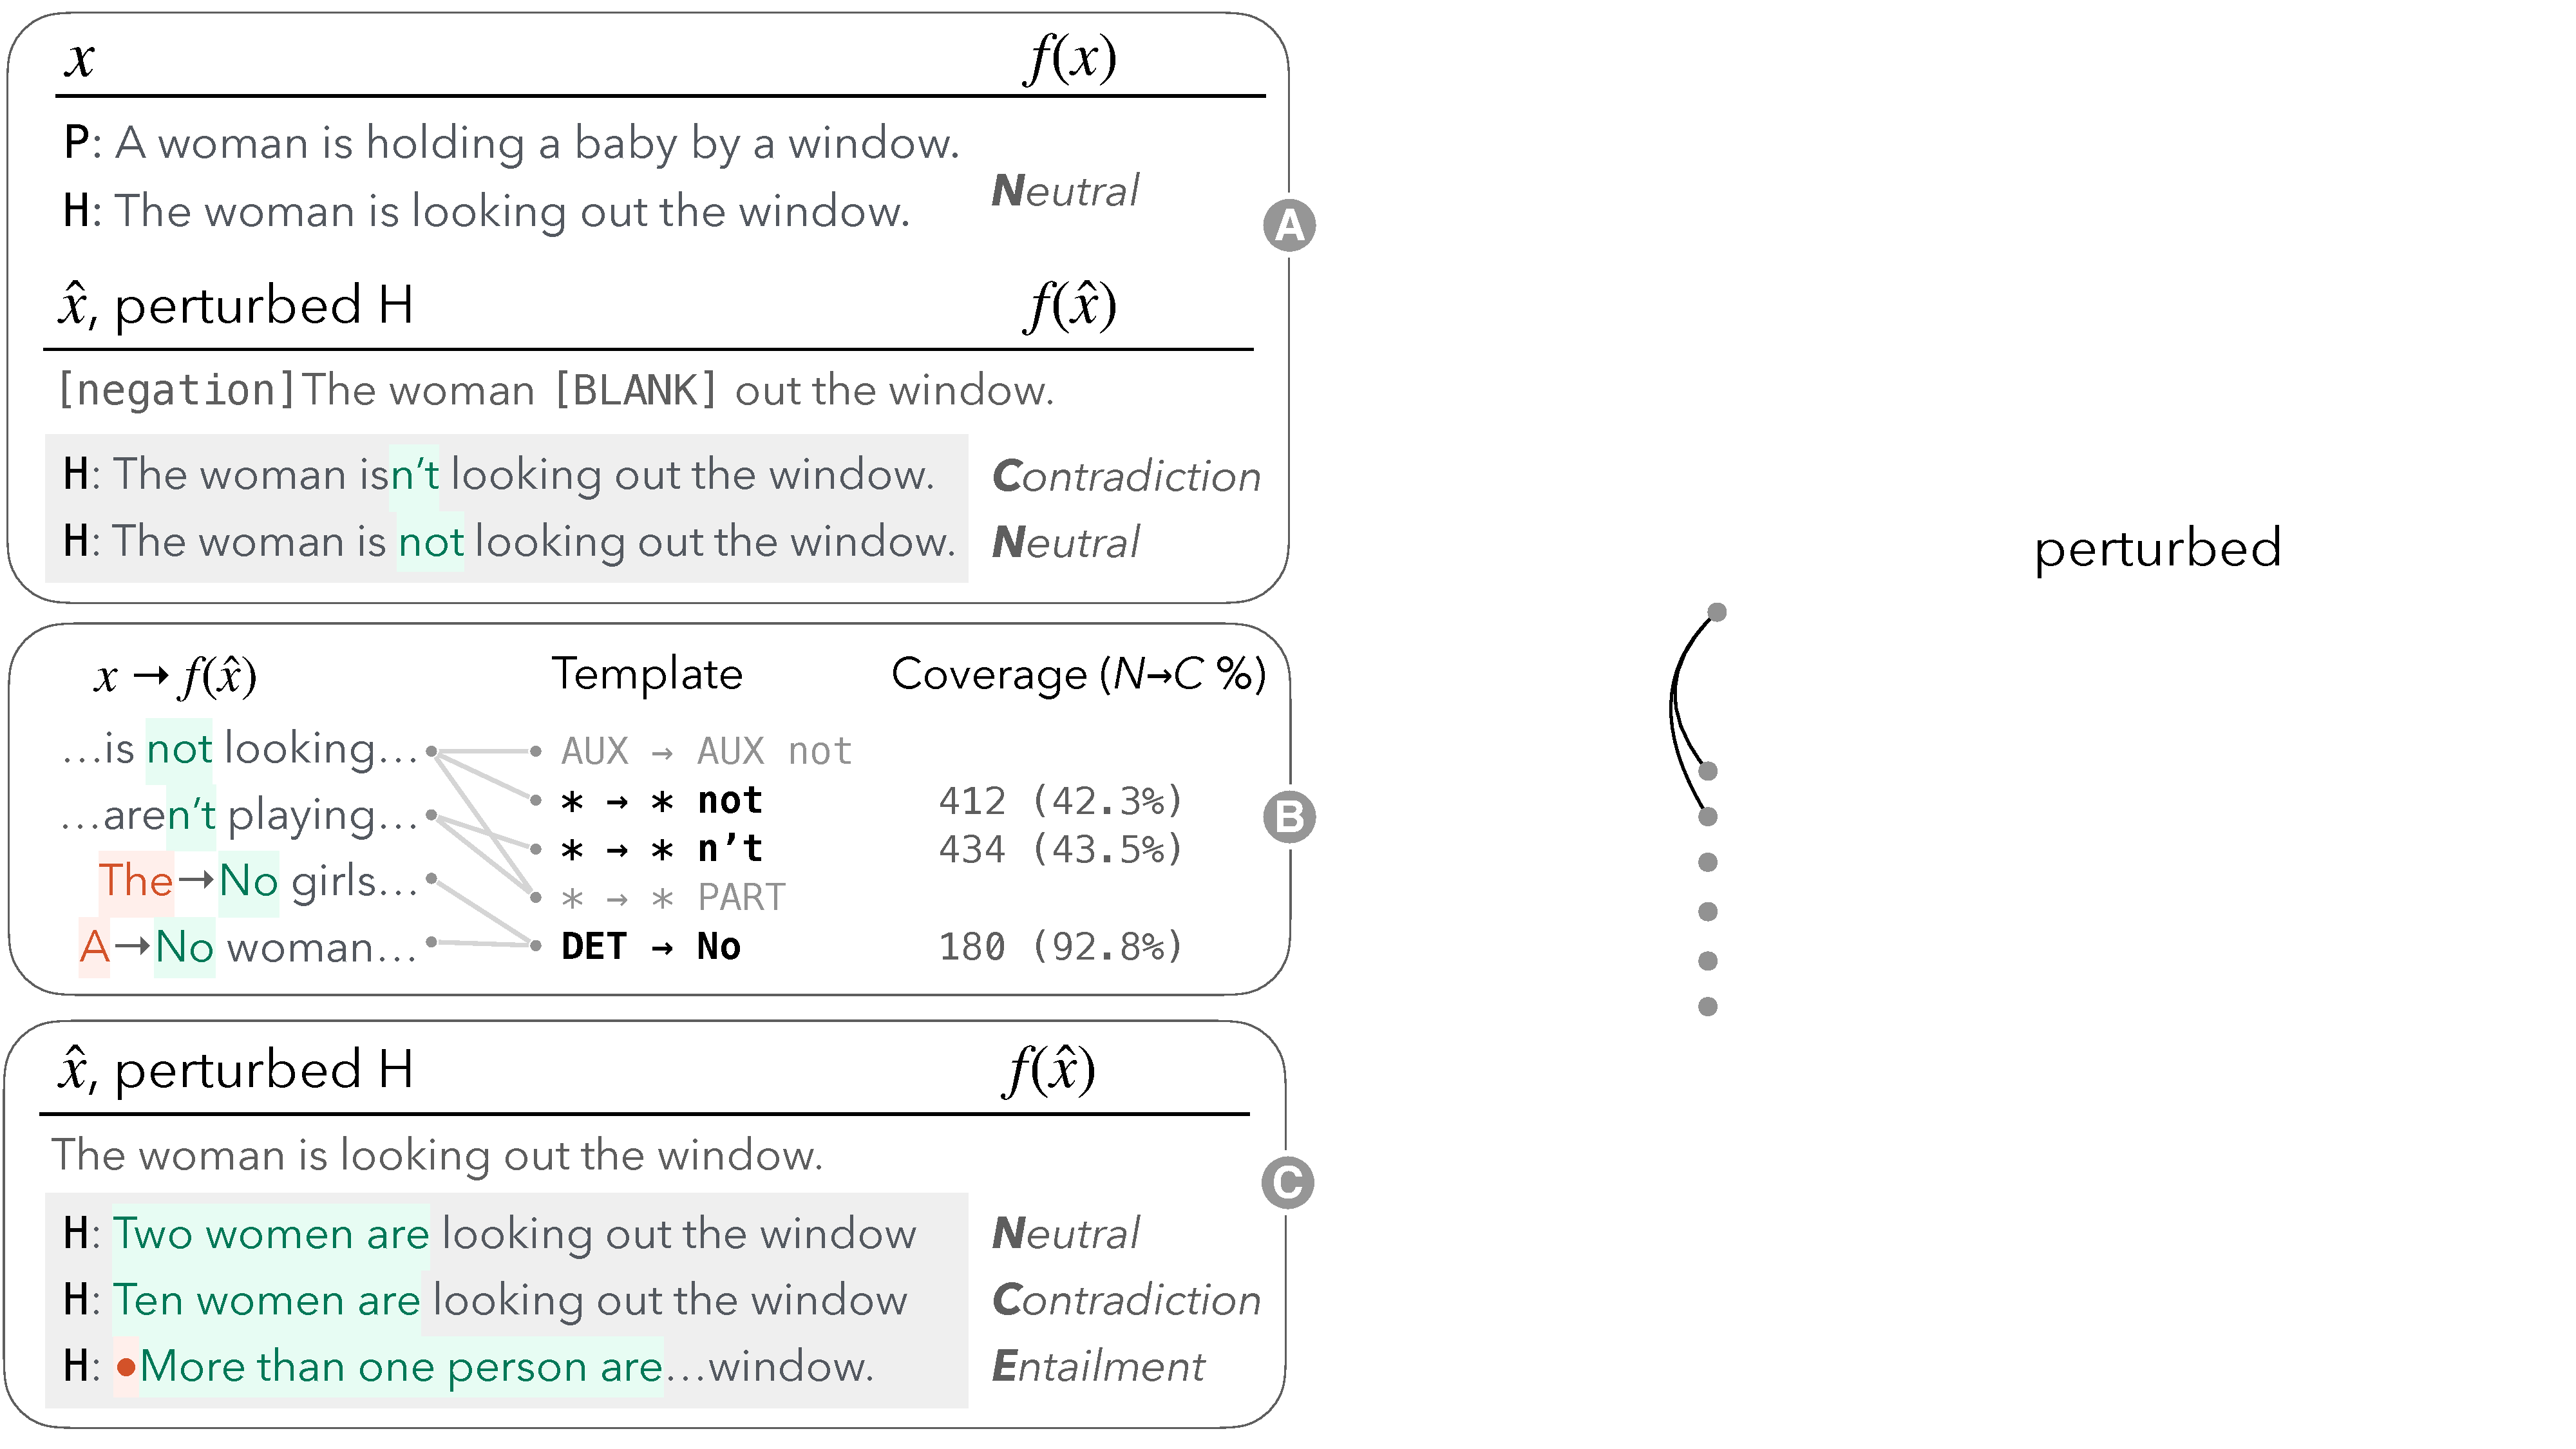
\includegraphics[trim={0 12.5cm 33cm 0cm},clip,width=1\columnwidth]{figures/err_analysis.pdf}
\vspace{-15pt}
\caption{
(A) An \nli case with a \emph{Neutral} prediction (\uline{underlined} $f(\xp)$ are correct).
\sysname generates counterfactual hypotheses conditioned on the \texttt{negation} \tagstr. 
(B) Generalizing perturbations into patterns~\cite{wu2020tempura}. The change \swap{\texttt{DET}}{no} flips $92.8\%$ of predictions from \emph{N}eutral~$\veryshortarrow$~\emph{C}ontradiction.
%(C) Another blank placement that leads to analyses on \emph{quantifiers}.
}
\vspace{-5pt}
\label{fig:err_analysis}
\end{figure}


To verify if the pattern is widespread, we generate counterfactuals with the \texttt{negation} \tagstr for a random set of instances correctly predicted as \emph{Neutral} ($n=895$). To generalize individual changes into patterns, we extract frequent \emph{counterfactual templates} with Tempura~\cite{wu2020tempura} (details in Appendix~\ref{appendix:err_analysis_template}), shown in Figure~\ref{fig:err_analysis}B.
The top templates (in bold) show that the model flips its prediction from \emph{Neutral} to \emph{Contradiction} with roughly the same frequency (${\approx}43\%$) whether the negation word is ``not'' or ``n't'', but flips much more frequently with a different negation pattern where a determiner is replaced with ``no'' ($92.8\%$). While these behaviors may be correct in some instances, they often are not (\eg Figure~\ref{fig:err_analysis}A), and thus would warrant further exploration, and potential mitigation strategies (\eg counterfactual training, \S\ref{sec:app_label}).
Tangentially, the impact of \swap{\texttt{DET}}{no} might lead the analyst to explore the impact of perturbing the \emph{subject} of hypotheses, which we do in Figure~\ref{fig:err_analysis_quantifier} by placing a \texttt{[BLANK]} on the subject rather than using a control code.
This leads to the discovery of unstable and erroneous behaviors regarding \emph{quantifiers}, which we analyze in more detail in Appendix~\ref{appendix:err_analysis_quantifier_case}.




\begin{figure}[t]
\centering
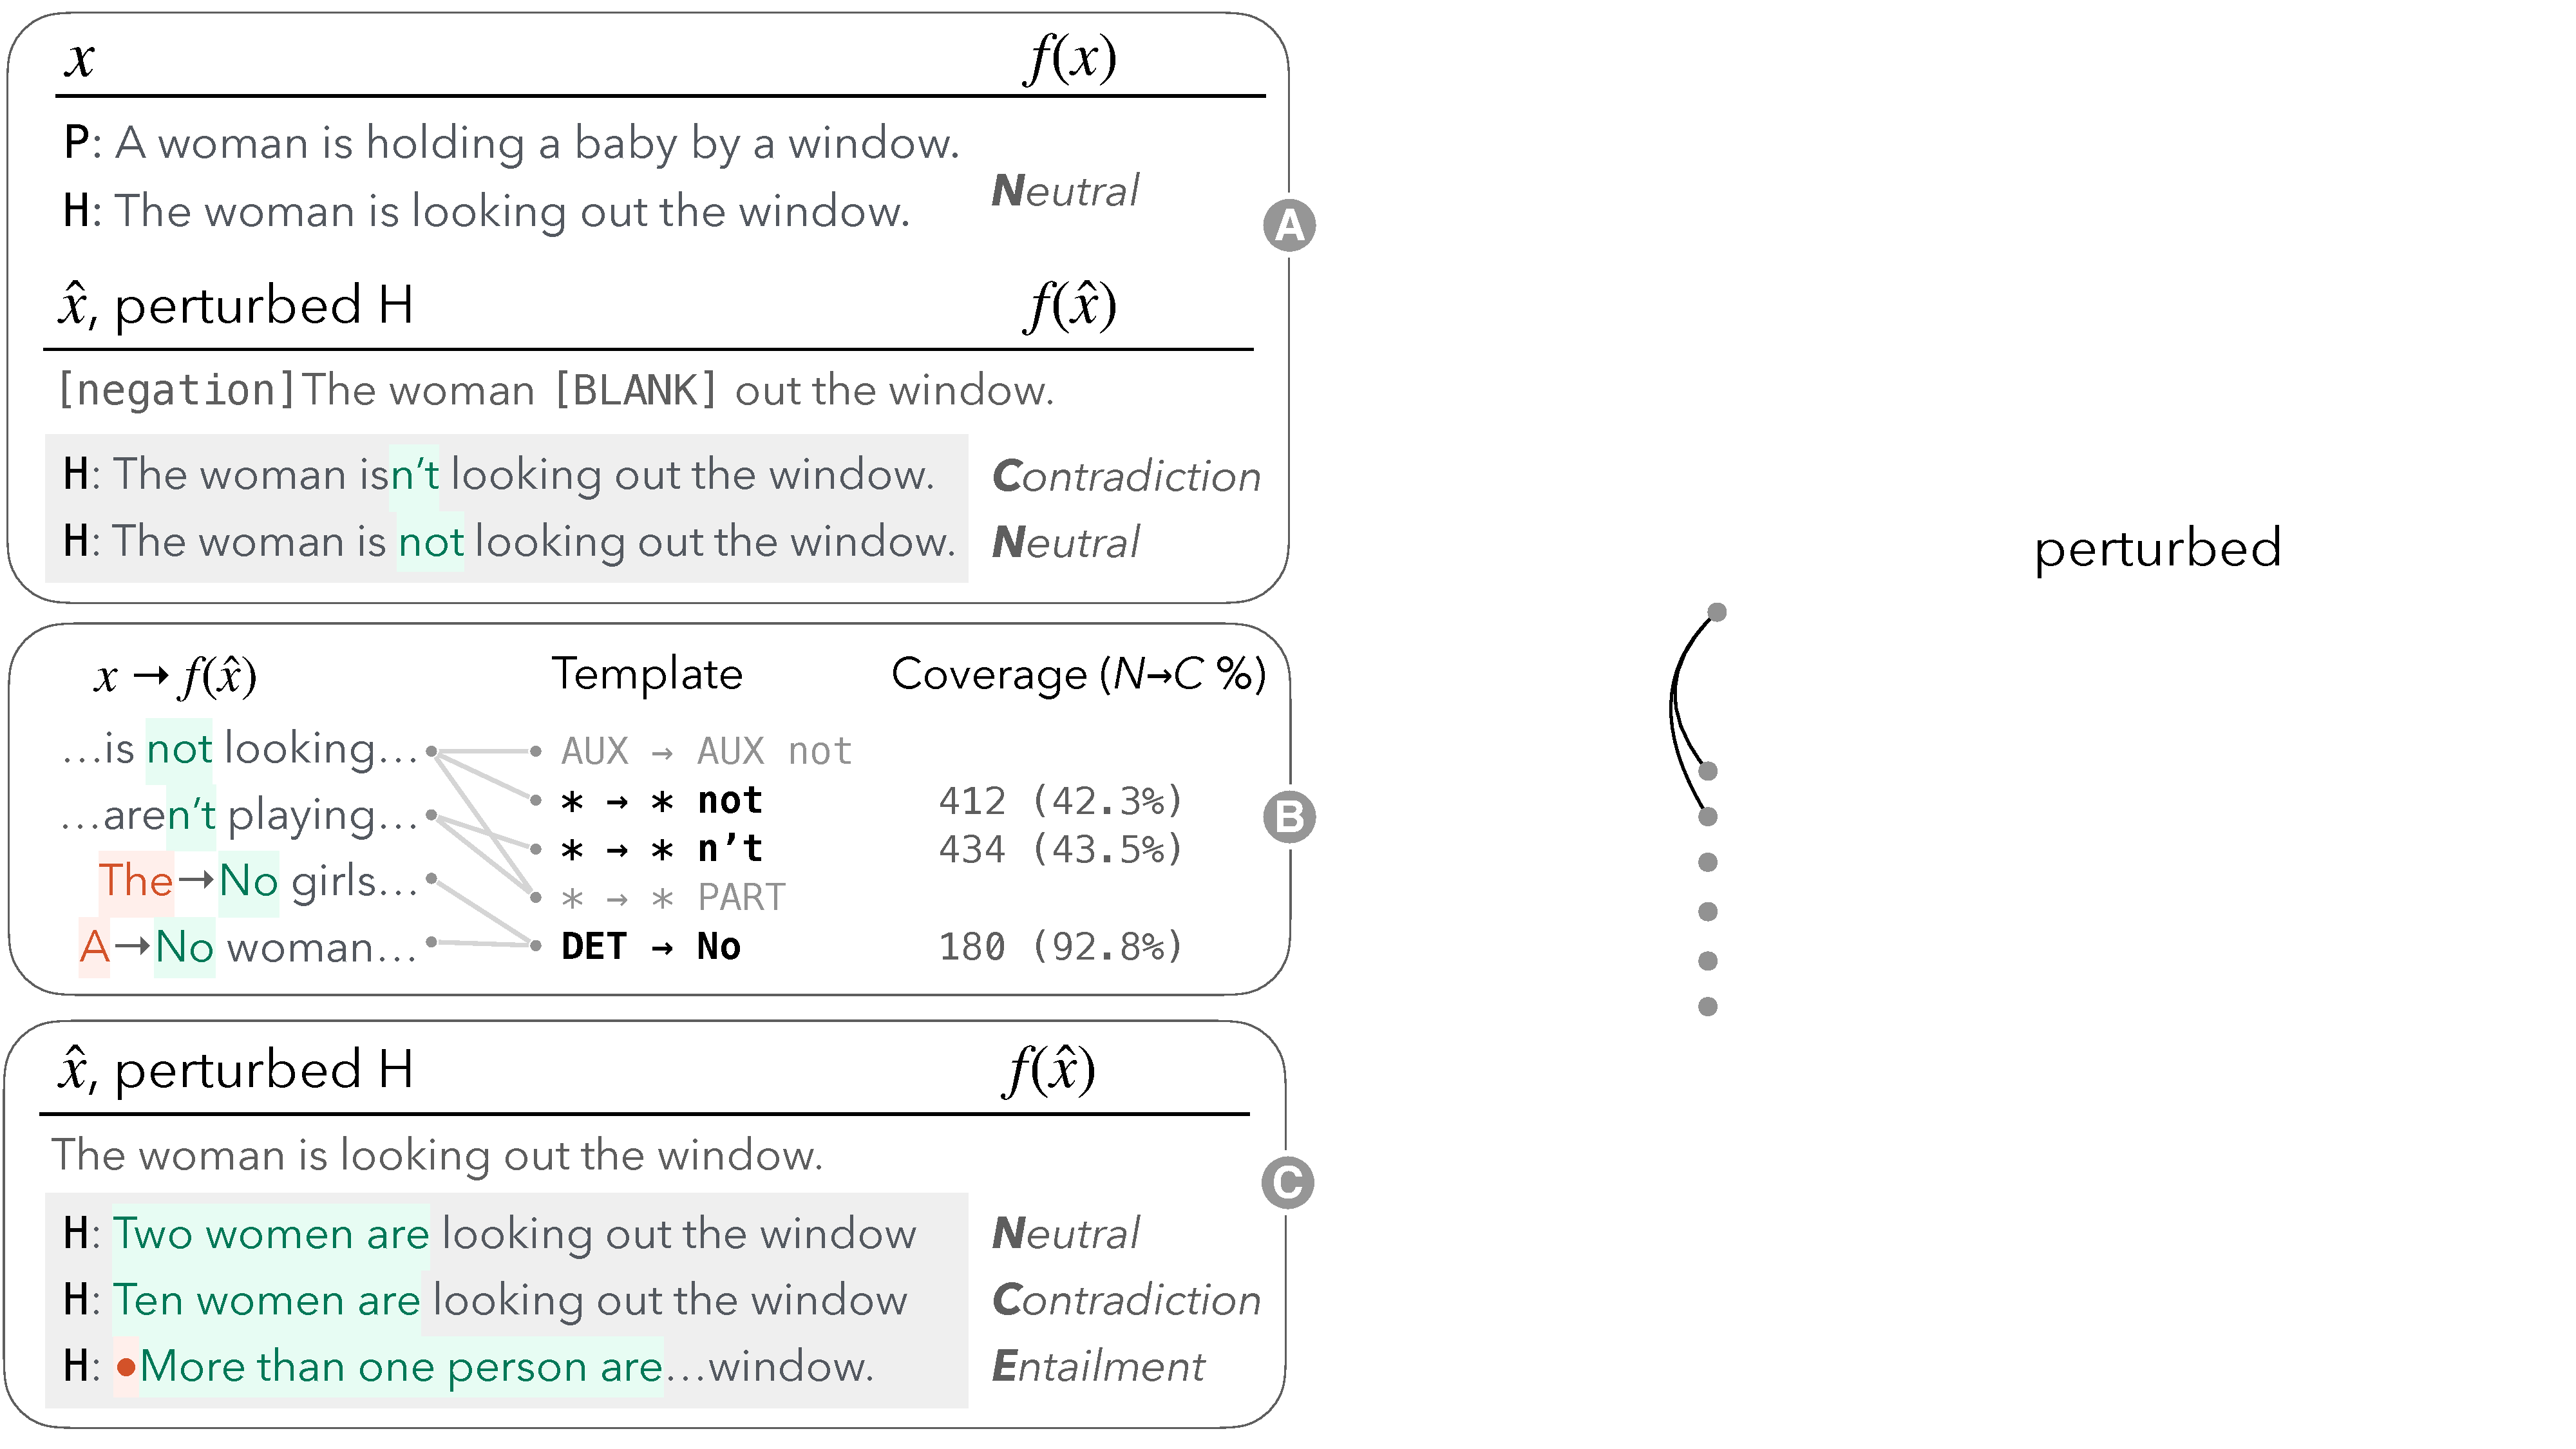
\includegraphics[trim={0.5cm 1.5cm 32.5cm 25.5cm}, clip,width=1\columnwidth]{figures/err_analysis.pdf}
\vspace{-15pt}
\caption{
Perturbing the subject of $x$ in Figure~\ref{fig:err_analysis}A through \texttt{[BLANK]}, resulting in erroneous predictions for different \emph{quantifiers}
(all should be \uline{\emph{Neutral}}). 
}
\vspace{-10pt}
\label{fig:err_analysis_quantifier}
\end{figure}

\paragraph{Discussion.} 
\sysname{} is a powerful tool for interactive analysis.
Generating multiple counterfactuals per instance leads to insights that might be missed by manual analysis, and the controls provided by \tagstrs and \texttt{[BLANK]}s allow for analyses that would be non-trivial to do manually~\cite{wu2019errudite} or with masked language models (\eg Figure~\ref{fig:err_analysis}B places negations in various parts of sentences, and Figure~\ref{fig:err_analysis_quantifier} replaces spans with other spans of varying lengths). Besides error analysis, an analogous interactive use of \sysname{} may be suitable for test creation~\cite{checklist:acl20} and forms of data augmentation that are more guided than what we presented in \S\ref{sec:app_label}.
